% -*- coding: utf-8 -*-
\documentclass[11pt]{article}
\usepackage[UTF8]{ctex}
\usepackage{graphicx}
\usepackage[a4paper, body={18cm,22cm}]{geometry}
\usepackage{amsmath,amssymb,amstext,wasysym,enumerate,graphicx}
\usepackage{float,abstract,booktabs,indentfirst,amsmath}
\usepackage{array}
\usepackage{booktabs}
\usepackage{multirow}
\usepackage{diagbox}
\renewcommand\arraystretch{1.4}
\usepackage{indentfirst}
\usepackage{caption}
\usepackage[colorlinks,linkcolor=blue]{hyperref}
\usepackage{algorithm}
\usepackage{algorithmicx}
\usepackage{algpseudocode}
\setlength{\parindent}{2em}

\geometry{left=2.8cm,right=2.2cm,top=2.5cm,bottom=2.5cm}
%\geometry{left=3.18cm,right=3.18cm,top=2.54cm,bottom=2.54cm}

\title{\LARGE \bf 可交互多视图可视化作业报告}
\author{\LARGE 张启哲 \quad 1900011638}
\date{\Large \today}

\begin{document}
	\maketitle
	
	\begin{figure}[h]
		\centering
		
\includegraphics[width=8cm]{../Figure/pku.jpg}
	\end{figure}
	
	\renewcommand{\contentsname}{目录(Contents)}
	\renewcommand{\algorithmicrequire}{\textbf{Input:}}
	\renewcommand{\algorithmicensure}{\textbf{Output:}}
	
	\tableofcontents
	
	\thispagestyle{empty}
	
	\newpage
	
	\setcounter{page}{1}
	
	\section{数据描述与维度分析(Data Description \& Dimension Analysis)}
	\subsection{数据描述}
	本次可视化作业使用的数据是来自于\href{https://projects.iq.harvard.edu/cbdb/data-sets}{China Biographical Database Project(CBDB)}中Ming Jinshi List的明进士数据。数据集包括明代52年科举考试的所有进士原始资料,共14116人。
	
	数据集以excel数据xlsx的格式呈现,共有3个工作表。第1个工作表Ming Jinshi Lists中包括了所有进士的详细信息,第2个工作表Release Notes中描述了3个工作表中的内容并列出了各次科举考试的年份和资料出处,第3个工作表dazi rule描述了进士数据项的格式。
	
	\subsection{维度分析}
	数据集中的数据项包含了出处、年份、姓名、甲次、名次、籍贯、户籍、科目、年龄等诸多属性,而部分属性在某些年份的数据存在缺失,故本次多视图可视化项目主要采用了数据完整的5个属性(年份、户籍、科目、甲次与籍贯)作为分析与展示的维度。
	
	年份维度:1592年的进士户籍记录有明显异常,可视化结果中不予展示,其余年份的数据无误,但与数据集给出的52年这一数字有偏差,除去1592年剩余共50个年份;户籍维度:根据《明史》、《后湖志》等古籍记载,明代的户籍主要分为军、民、匠、灶四类,考虑到数据集本身的记录,本项目将进士户籍共分为民、军、官、匠、灶5类;科目维度:按照科举考试的常规科目五经分为诗、书、礼、易、春秋5类;甲次维度:按照科举考试结果分为一、二、三甲,其中一甲共3人,第一名为状元,第二名为榜眼,第三名为探花,二甲每年为十几人到一百多人不等,三甲则为一百人到三百多人不等,最多不超过三百五十人;籍贯维度:按照明代行政区划分为了司、府两个行政级别,其中司17个、府146个。
	
	数据分析时将年份与户籍类型组织在一起,可以了解到考生户籍类型随时间的分布情况,有助于分析明代各社会阶层在不同年代的生存与发展状况;将考试科目与甲次组织在一起,可以了解到各考试科目的热门程度以及对不同分段考生的偏差;籍贯维度单独呈现,分为司、府两个级别,展示社会精英的地域分布特点,也反映出各地区的教育水平差异。
	
	\section{设计目标与宗旨(Design Objective)}
	本项目的设计目标是通过多视图的形式将不同维度有机结合,并通过不同视图之间的交互动态地分析高维数据,宗旨是结构清晰、布局合理、操作简洁。
	
	具体设计方面,采用了3个视图结合的方式布局。整个画布的左上角通过堆叠面积图(StackedAreachart)的形式将年份与户籍类型两个维度结合查看,右上角通过堆叠柱状图(StackedBarchart)的形式将考试科目与中举甲次两个维度结合查看,下方则通过矩形树图(SquarifiedTreemap)的形式呈现进士的籍贯分布,有司、府两个行政级别可以切换。
	
	上方的2个视图可以通过点击交互互相控制,而下方的树图则可以同时控制上方的视图。下面具体介绍3个视图以及交互设计。
	
	\subsection{堆叠面积图}
	\begin{figure}[H]
		\centering
		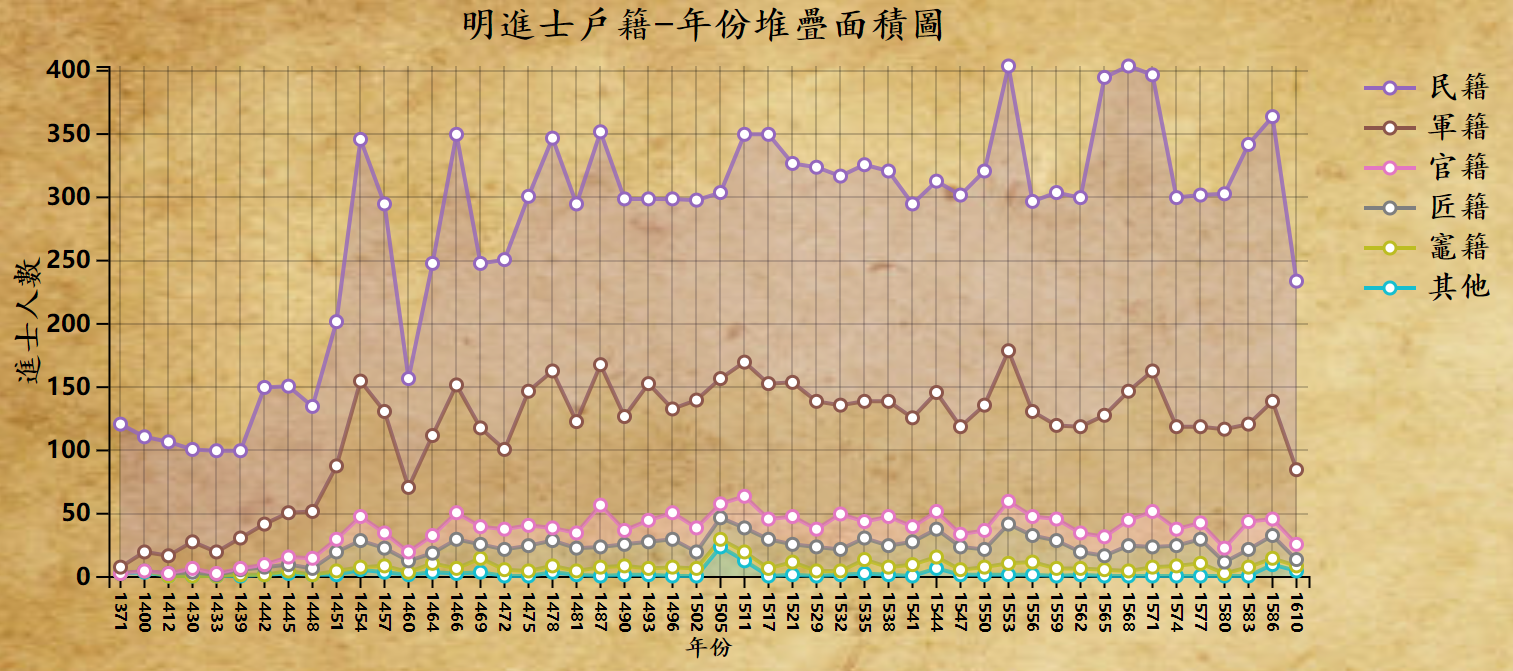
\includegraphics[width=12.5cm]{../Figure/StackedAreachart.png}
		\caption{户籍-年份堆叠面积图}
	\end{figure}
	
	堆叠面积图中,横轴为年份,从1371-1610共划分为50次,纵轴为进士人数,按照其他-灶籍-匠籍-官籍-军籍-民籍的顺序从下到上堆叠,不同颜色代表了不同的户籍种类,每个小圆圈代表一个数据点,线与线之间的距离代表了该类户籍的进士人数,面积表示该户籍的总人数,而最高点则表示了当年考取的进士总人数。

	\subsection{堆叠柱状图}
	\begin{figure}[H]
		\centering
		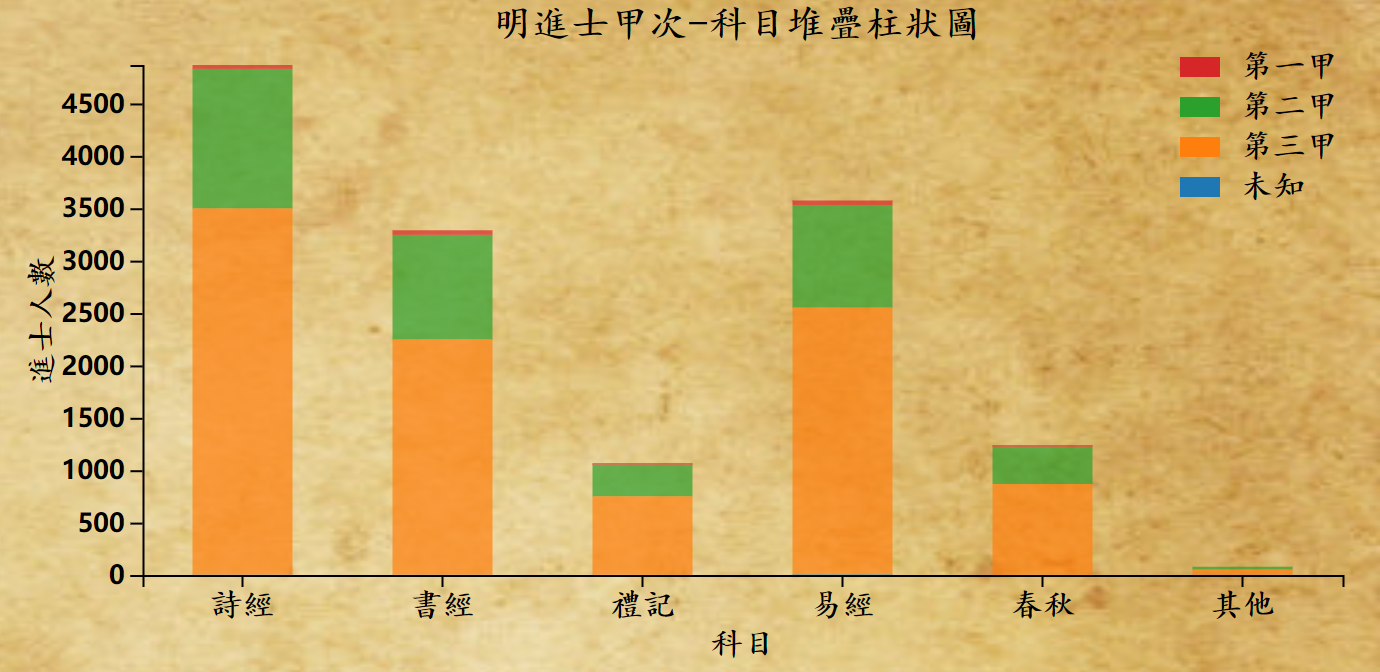
\includegraphics[width=12.5cm]{../Figure/StackedBarchart.png}
		\caption{甲次-科目堆叠柱状图}
	\end{figure}

	堆叠柱状图中,横轴为考试科目,共有诗经、书经、礼记、易经、春秋与其他6类,纵轴为进士人数,按照未知-第三甲-第二甲-第一甲的顺序从下到上堆叠,不同颜色代表了不同的甲次,柱子的总高度则代表了该考试科目下考取的进士总人数。

	\subsection{矩形树图}
	\begin{figure}[H]
		\centering
		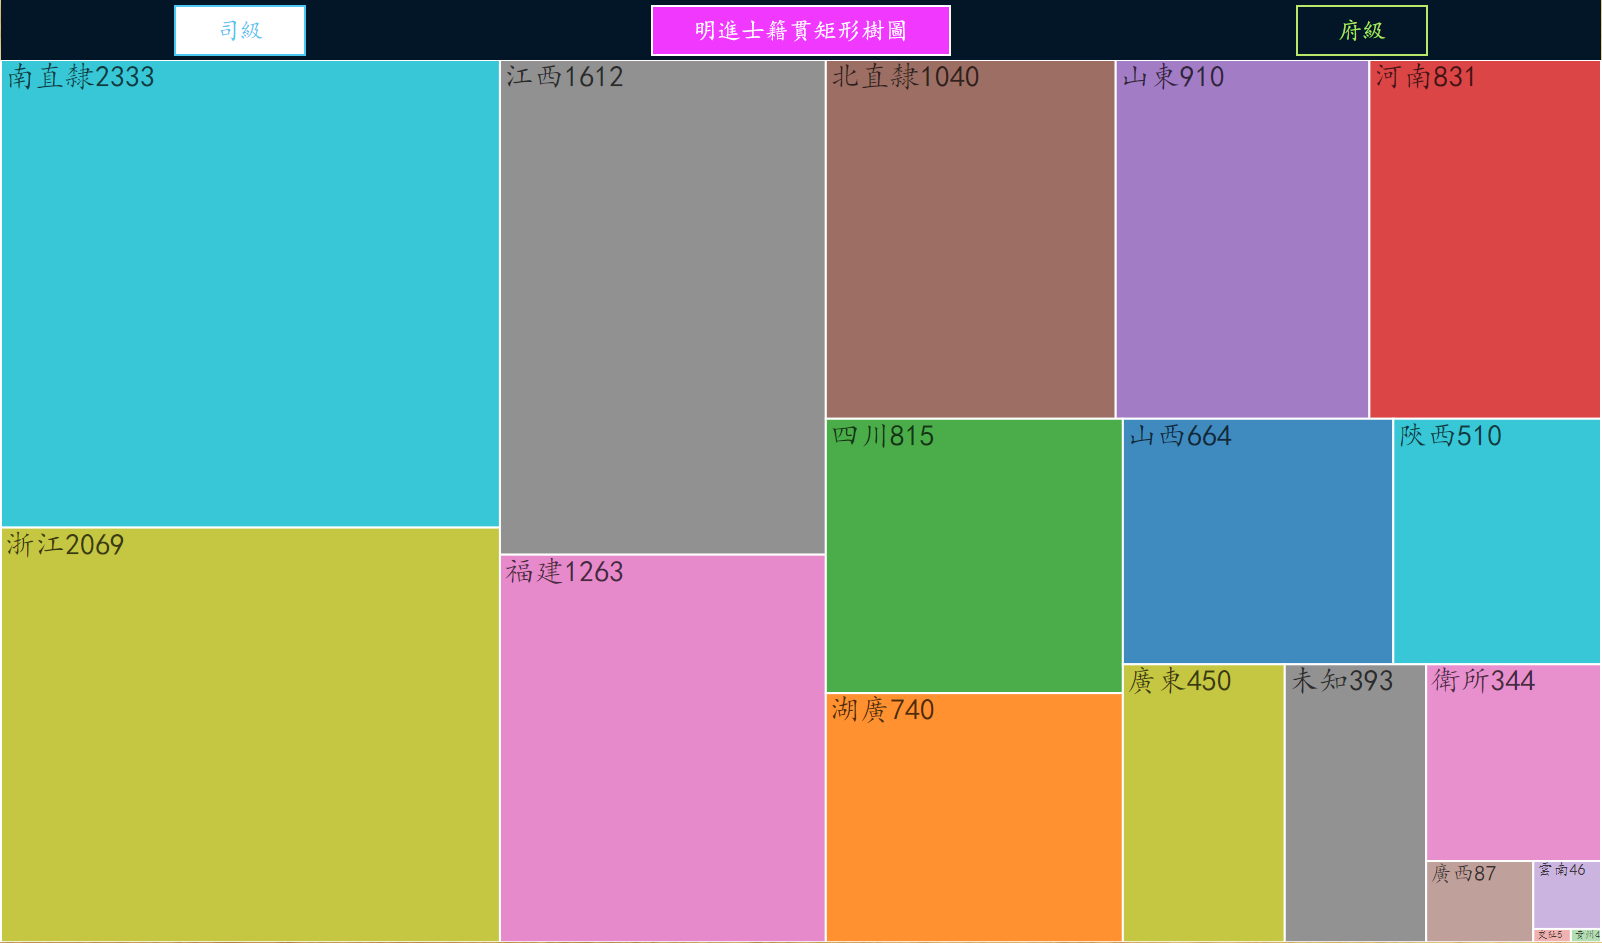
\includegraphics[width=12.5cm]{../Figure/SquarifiedTreemap.png}
		\caption{籍贯矩形树图}
	\end{figure}
	
	矩形树图中,通过SquarifiedTreemap可视化了按照行政区划层次结构组织的进士数据,分为司、府两个行政等级,可以点击切换。
	
	\subsection{交互设计}
	\begin{figure}[h]
		\begin{minipage}[h]{0.5\linewidth}
			\centering
			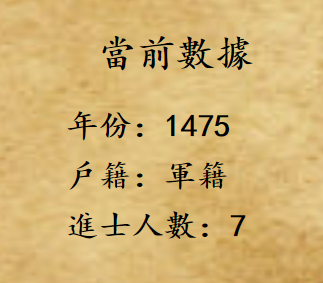
\includegraphics[height=3cm]{../Figure/nowData.png}
			\caption{动态数据项显示}
		\end{minipage}
		\begin{minipage}[h]{0.5\linewidth}
			\centering
			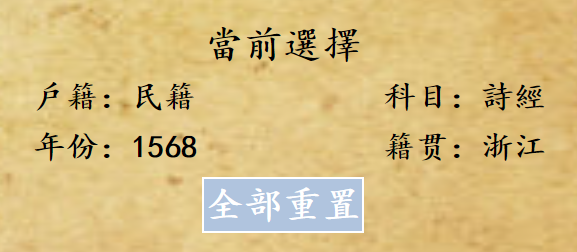
\includegraphics[height=3cm]{../Figure/nowChoice.png}
			\caption{刷选帮助显示}
		\end{minipage}
	\end{figure}

	动态数据项:当鼠标移至数据项上时,画布左侧会显示对应数据项内容:堆叠面积图(年份、户籍、进士人数)、堆叠柱状图(科目、甲次、进士人数)、矩形树图(行政级别、行政区划、进士人数)。
	
	动态刷选交互:鼠标点击堆叠面积图上的小圆圈时,右侧堆叠柱状图会按照对应年份筛选;点击不同颜色面积区域时,右侧堆叠柱状图会按照对应户籍类型筛选;点击堆叠柱状图中的立柱时,左侧堆叠面积图会按照对应考试科目筛选;点击下方矩形树图中的小矩形时,上方2个视图均会按照对应行政级别与地区进行筛选。同时,树图上方的司、府级切换按钮可切换不同行政级别;上方的4个与右侧的1个重置按钮均可重置筛选条件。
	
	\section{可视化结果描述(Visualization Result Description)}
	\subsection{结果展示}
	代码库已上传至github: \href{https://github.com/Theia-4869/Interactive-Multiple-Views}{Theia-4869/Interactive-Multiple-Views}。
	
	\begin{figure}[H]
		\centering
		\includegraphics[width=11cm]{../Figure/figure.png}
		\caption{可交互多视图明进士数据可视化}
	\end{figure}
	
	
	\subsection{总结与分析}
	从数据集的统计结果来看,1451年后进士数量迅速增长,从之前的每年100人作业增长到300人以上并在以后基本保持稳定,进士人数最多的年份为1568年,共403人,最少的则为1433和1439年并列,仅有99人。户籍为民籍的考生有8404人,占全部考生的60\%,军籍次之,占到28\%,其余户籍的考生就较少了,这可能是由于科举考试是改变民籍百姓的几乎唯一出路,参军的青年大多身体素质较好但成绩和思维能力就相对差些,官家的小孩无论成绩如何在看重阶级身份与血统的社会都可以衣食无忧,而匠籍与灶籍的百姓平日则要承受繁重的劳役,加之经济情况不好,很难拥有参加科举考试的机会和条件。从考试科目来看,选择诗经的考生最多,达到了4867人,占34\%,易经与书经次之,占23\%$\sim$25\%,春秋与礼记最少,只占到8\%左右,值得一提的是,一甲率最高的科目不是选择人数最多的诗经,而是书经(1.3\%)与易经(1.2\%),这大概是因为诗经科目较为常规,难有新意,书经和易经有时更能给考官带来惊喜,而选择人数过少的春秋和礼记则较难。而考生的地域分布依然与今日的全国教育格局类似,南方沿海地区教育水平高,中举人数多,西北部和偏远地区则相对落后,进士人数较少。
	
	从多视图的交互来看,不同年份与户籍的考生在考试科目的选择上基本一致,都是诗经>书经、易经>礼记、春秋,这可能与不同典籍的内容及考试的题目类型有关,是长期的考试经验决定的,数据也证明了这一点,在1460年之前选择各科目考生的数量比例还时有波动,但1460年后比例基本稳定。从单个科目来看,春秋在早间年更受考生们的偏爱,而易经则成为了后来考生的坚定选择。地域分布方面,同样是南方考生的程度由于北方,进士人数多,一甲人数也多,而各地区考生在户籍类型的分布上也与全国平均水平相近(除卫所这一特殊的军籍管理行政机构外),又从另一个侧面证明了上文中解释的合理性。
	
	从整体设计来看,整体布局与操作较为简洁,可以考虑采用更多的视图与不同的图表类型展示不同维度数据之间的关系,也可以添加更多的交互机制为用户分析数据提供便捷与选择。
	
\end{document}

%%%%%%%%%%%%%%%%%%%%%%%%%%%%Library%%%%%%%%%%%%%%%%%%%%%%%%%%%%%%%%%%%%%%%

% 1. 脚注用法
LaTeX\footnote{Latex is Latex} is a good software

%2. 强调
\emph{center of percussion} %[Brody 1986], %\lipsum[5]

%3. 随便生成一段话
\usepackage{lipsum}
\lipsum[4]

%4. 列条目
\begin{itemize}
	\item the angular velocity of the bat,
	\item the velocity of the ball, and
	\item the position of impact along the bat.
\end{itemize}

%5. 表格
\begin{table}[h]
	\centering  
	\begin{tabular}{c|cc}
		\hline
		年份 & \multicolumn{2}{c}{指标}\\
		\hline
		2017 & 0.9997 & 0.0555 \\
		2018 & 0.9994 & 0      \\
		2019 & 0.9993 & 0      \\
		\hline
	\end{tabular}
	\caption{NAME}\label{SIGN}
\end{table}

\begin{center}
	\begin{tabular}{c|cclcrcc}
		\hline
		Year & theta & $S_1^-$ & $S_2^-$ & $S_3^-$ & $S_4^+$ & $S_5^+$ & $S_6^+$ \\%表格标题
		\hline
		2016 & 1      & 0      & 0 & 0.0001 & 0      & 0      & 0 \\
		2017 & 0.9997 & 0.0555 & 0 & 0.2889 & 0.1844 & 0.463  & 0 \\
		2018 & 0.9994 & 0      & 0 & 0.0012 & 0.3269 & 0.7154 & 0 \\
		2019 & 0.9993 & 0      & 0 & 0      & 0.4325 & 1.0473 & 0 \\
		2020 & 0.9991 & 0      & 0 & 0      & 0.5046 & 1.2022 & 0 \\
		2021 & 0.999  & 0      & 0 & 0      & 0.5466 & 1.2827 & 0 \\
		2022 & 0.9989 & 0.0017 & 0 & 0.3159 & 0.562  & 1.2995 & 0 \\
		2023 & 0.9989 & 0      & 0 & 0.0109 & 0.5533 & 1.2616 & 0 \\
		2024 & 0.9989 & 0      & 0 & 0      & 0.5232 & 1.1769 & 0 \\
		2025 & 0.9989 & 0      & 0 & 0.1009 & 0.4738 & 1.0521 & 0 \\
		2026 & 0.9991 & 0      & 0 & 0      & 0.4071 & 0.8929 & 0 \\
		2027 & 0.9992 & 0.0004 & 0 & 0.1195 & 0.3248 & 0.7042 & 0 \\
		2028 & 0.9994 & 0.0164 & 0 & 0.046  & 0.2287 & 0.4902 & 0 \\
		2029 & 0.9997 & 0      & 0 & 0.0609 & 0.12   & 0.2545 & 0 \\
		2030 & 1      & 0      & 0 & 0      & 0      & 0      & 0 \\
		\hline
	\end{tabular}
\end{center}

%6. 数学公式
\begin{equation}
	a^2 = a * a\label{aa}
\end{equation}

\[
\begin{pmatrix}{*{20}c}
	{a_{11} } & {a_{12} } & {a_{13} }  \\
	{a_{21} } & {a_{22} } & {a_{23} }  \\
	{a_{31} } & {a_{32} } & {a_{33} }  \\
\end{pmatrix}
= \frac{{Opposite}}{{Hypotenuse}}\cos ^{ - 1} \theta \arcsin \theta
\]

\[
p_{j}=\begin{cases} 0,&\text{if $j$ is odd}\\
	r!\,(-1)^{j/2},&\text{if $j$ is even}
\end{cases}
\]


\[
\arcsin \theta  =
\mathop{{\int\!\!\!\!\!\int\!\!\!\!\!\int}\mkern-31.2mu
	\bigodot}\limits_\varphi
{\mathop {\lim }\limits_{x \to \infty } \frac{{n!}}{{r!\left( {n - r}
			\right)!}}} \eqno (1)
\]

%7. 双图并行
\begin{figure}[h]
	% 一个2*2图片的排列
	\begin{minipage}[h]{0.5\linewidth}
		\centering
		\includegraphics[width=0.8\textwidth]{./figures/0.jpg}
		\caption{Figure example 2}
	\end{minipage}
	\begin{minipage}[h]{0.5\linewidth}
		\centering
		\includegraphics[width=0.8\textwidth]{./figures/0.jpg}
		\caption{Figure example 3}
	\end{minipage}
\end{figure}

%8. 单张图片部分
\begin{figure}[h]
	%\small
	\centering
	\includegraphics[width=12cm]{./figures/mcmthesis-aaa.eps}
	\caption{Figure example 1} \label{fig:aa}
\end{figure}

%%%%%%%%%%%%%%%%%%%%%%%%%%%%%%%%%%%%%%%%%%%%%%%%%%%%%%%%%%%%%%%%%%%%%%%%%%%%%
\begin{minipage}{0.5\linewidth}
	\begin{tabular}{|c|c|c|}
		\hline
		\multicolumn{2}{|c|}{\multirow{2}{*}{合并}}&测试\\
		\cline{3-3}
		\multicolumn{2}{|c|}{}& 0.9997  \\
		\hline
		2019 & 0.9993 & 0 \\
		\hline
	\end{tabular}
\end{minipage}

\begin{minipage}{0.5\linewidth}
	\begin{tabular}{c|ccc}
		\hline
		年份 & \multicolumn{3}{c}{指标}\\
		\hline
		\multirow{3}{*}{合并}&2017 & 0.9997 & 0.0555 \\
		&2018 & 0.9994 & 0      \\
		&2019 & 0.9993 & 0      \\
		\hline
	\end{tabular}
\end{minipage}

\begin{table}[h]
	\centering	
	\begin{Large}
		\begin{tabular}{p{4cm} p{8cm} < {\centering}}
			\hline
			院\qquad 系: & 信息工程学院 \\
			\hline
			团队名称: & PlantBook Team \\
			\hline
			分\qquad 组: & 第0组1号 \\
			\hline
			日\qquad 期: & 2017年10月28日 \\
			\hline
			指导教师: & 吱吱吱\\
			\hline
		\end{tabular}
	\end{Large}
\end{table}

\ctexset{
	section={
		format+=\heiti \raggedright,
		name={,、},
		number=\chinese{section},
		beforeskip=1.0ex plus 0.2ex minus .2ex,
		afterskip=1.0ex plus 0.2ex minus .2ex,
		aftername=\hspace{0pt}
	},
}

\begin{table}[h]
	\centering
	\begin{Large}
		\begin{tabular}{p{3cm} p{7cm}<{\centering}}
			院  \qquad  系: & 信息工程学院           \\ \cline{2-2}
		\end{tabular}
	\end{Large}		
\end{table}
\thispagestyle{empty}
\newpage
\thispagestyle{empty}
\tableofcontents
\thispagestyle{empty}
\newpage
\setcounter{page}{1}

% 9. 代码
\usepackage{listings}
\usepackage{xcolor}
\lstset{
	numbers=left, 
	numberstyle= \tiny, 
	keywordstyle= \color{ blue!70},
	commentstyle= \color{red!50!green!50!blue!50}, 
	frame=shadowbox, % 阴影效果
	rulesepcolor= \color{ red!20!green!20!blue!20} ,
	escapeinside=``, % 英文分号中可写入中文
	xleftmargin=2em,xrightmargin=2em, aboveskip=1em,
	basicstyle=\footnotesize,
	framexleftmargin=2em
}
